\documentclass[10pt, journal]{IEEEtran}
\usepackage{graphicx}
\usepackage{amsmath}
\usepackage{cite}

\title{uFluidics Amplifier and DSP}
\author{Michael Nolan}
\begin{document}
\maketitle \par
\section{Amplifier}
\subsection{Specification}
Because the signal from the uFluidics device is so small, an extremely
low noise amplifier is needed to create a large enough signal that the
DSP can detect it. From the initial COMSOL simulations, it appeared
that the uFluidics pickup coil generated a voltage between 1 and
600nV. Since these voltages are approaching the limits of what can be
measured without massive research budgets, a 100nV signal from the
device was assumed. Next, for the signal to be input to the DSP, it
needs to be centered around 1.5V (half of the supply voltage), and to
have a relatively large swing of 200mV pk/pk. The 200mV swing gives
enough room that if the signal is really 600mV or larger the amplifier
will not saturate, but is also large enough to be easily detected by
the DSP. This means the amplifier needs a gain of
\begin{equation*}
  \frac{200mV}{100nV} = 2\cdot10^6V/V
\end{equation*}
Next, after some experimentation, it was determined that the DSP can
reliably detect a signal that has twice the amplitude of the
noise. Therefore, the amplifier's input noise needs to be less than
50nV pk/pk, and ideally should be less, to leave some room for the
uFluidics signal to be smaller than calculated.

\subsection{Component Selection}
After some research, the AD8428 low noise instrumentation amplifier
was selected as it had a very low input noise of 50nV, and multiple
amplifiers could be paralleled to reduce the noise even
further\cite{ad8428-parallel}. The AD8428 has a gain of 2000
V/V\cite{ad8428}, so another amplifier is needed after the AD8428. The
AD4528 op amp was selected for this task because of its low input
offset voltage and low noise. The AD4528 was set up to have a gain of
\begin{equation}
  \frac{2\cdot10^6}{2000} = 1000
\end{equation}
in a differential amplifier configuration to bring the total system
gain to $2\cdot10^6$ and to introduce the 1.5V offset needed to feed
the signal to the DSP.

\subsection{Schematic}

\begin{figure}[ht!]
  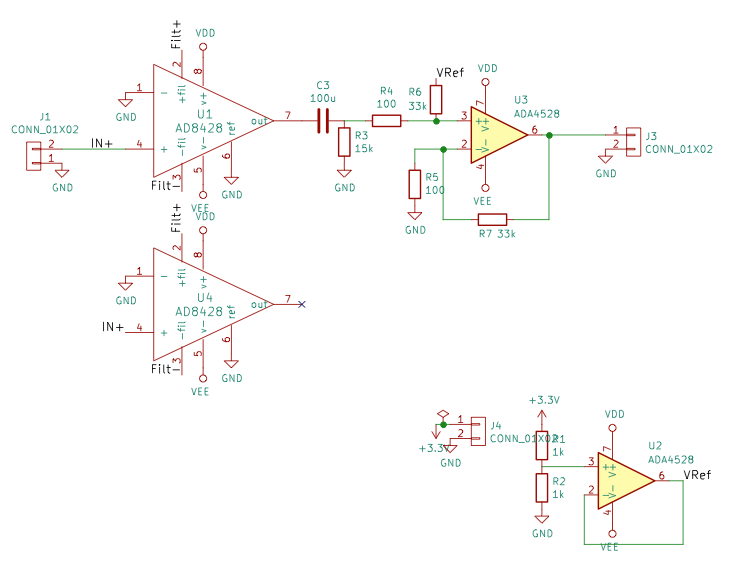
\includegraphics[width=8cm]{../photos/amp.png}
  \caption{Amplifier Schematic}
  \label{fig:amp}
\end{figure}

The amplifier uses two AD8428 instrumentation amplifiers to give an
input noise of $\frac{50nV}{\sqrt{2}}$\cite{ad8428-parallel}. Notice
how both ICs are connected to the input, and have their \texttt{filt+}
and \texttt{filt-} terminals connected, but only one has its output
connected to the rest of the circuit as described in
\cite{ad8428-parallel}. Next, the output of the AD8428 is connected to
a high pass filter with a cutoff of $\frac{1}{2\pi 100uF * 15k\Omega}
= 0.1Hz$ to remove any DC voltage from the input offset voltage of the
AD8428 or thermal effects from the uFluidics device. The filter then
connects to an opamp differential amplifier with a gain of 1000, with
a connection to the reference voltage $V_{ref}$. Finally, the
reference voltage $V_{ref}$ is generated by a resistor divider
feeding an opamp voltage buffer.

\section{Thermal Effects}
\subsection{Causes}
One of the effects observed when testing the Keithley nanovoltmeter
was a small voltage being generated across a thermal gradient. This
voltage was determined to be caused by the Seebeck Effect, where a
difference in temperature between two different metals causes a small
voltage to be generated \cite{seebeck}. In our device, the seebeck
effect is likely unavoidable, as there are multiple places where there
are dissimilar metals connected to each other between the uFluidics
coil and the amplifier IC.

\subsection{Mitigation}
However, the Seebeck Effect should not be much of a problem
directly. The amplifier already includes a high pass filter to remove
any voltage offset from the input amplifier's offset voltage, and the
voltage from the seebeck effect will only add or subtract from this
voltage. However, the Seebeck Effect has the capacity to introduce
noise that the high pass filter cannot remove, and it is this aspect
that must be mitigated. One of the ways that the Seebeck Effect could
introduce noise is from rapid thermal fluctuations somewhere in the
device. Therefore it may be adventageous to submerge all or part of
the device in a thermally conductive fluid such as mineral oil to
reduce this noise, even if it means introducing some voltage offset.

\section{DSP Portion}
Because the uFluidics device generates an extremely weak signal, when
the signal reaches the circuit to count the cells, it will have quite
a lot of noise in it. In order to accurately count the cells, the
signal will need to be processed in order to remove the noise and
detect when a cell passes through the device.

\subsection{DSP}
The DSP for this project needed to 
\begin{itemize}
\item Have a low cost
\item Have an on board ADC
\item Be more than able to process a 5ks/s signal (to allow for changes to processing algorithm)
\item Have enough ram to process the above signal in batches of 1024 samples
\item Be capable of driving a display or other peripherals to present results
\end{itemize}

After some searching, a dsPIC33f was determined to be able to fufill
the above requirements, and the dsPIC33FJ128GP802 was selected as it
had more than enough ram and processing power for our
use. Additionally, a less powerful DSP from the same product line
could be used in the final product after determining exactly how much
ram and processing power are needed.

\subsection{Processing}

According to \cite{dspguide}, the optimal way to separate a known
signal from white noise is to use correlation. Via COMSOL simulation
and via a crude prototype involving dropping a straw through a coil,
the signal of interest would have a shape similar to Figure
\,\ref{fig:input} \par
\begin{figure}[ht!]
  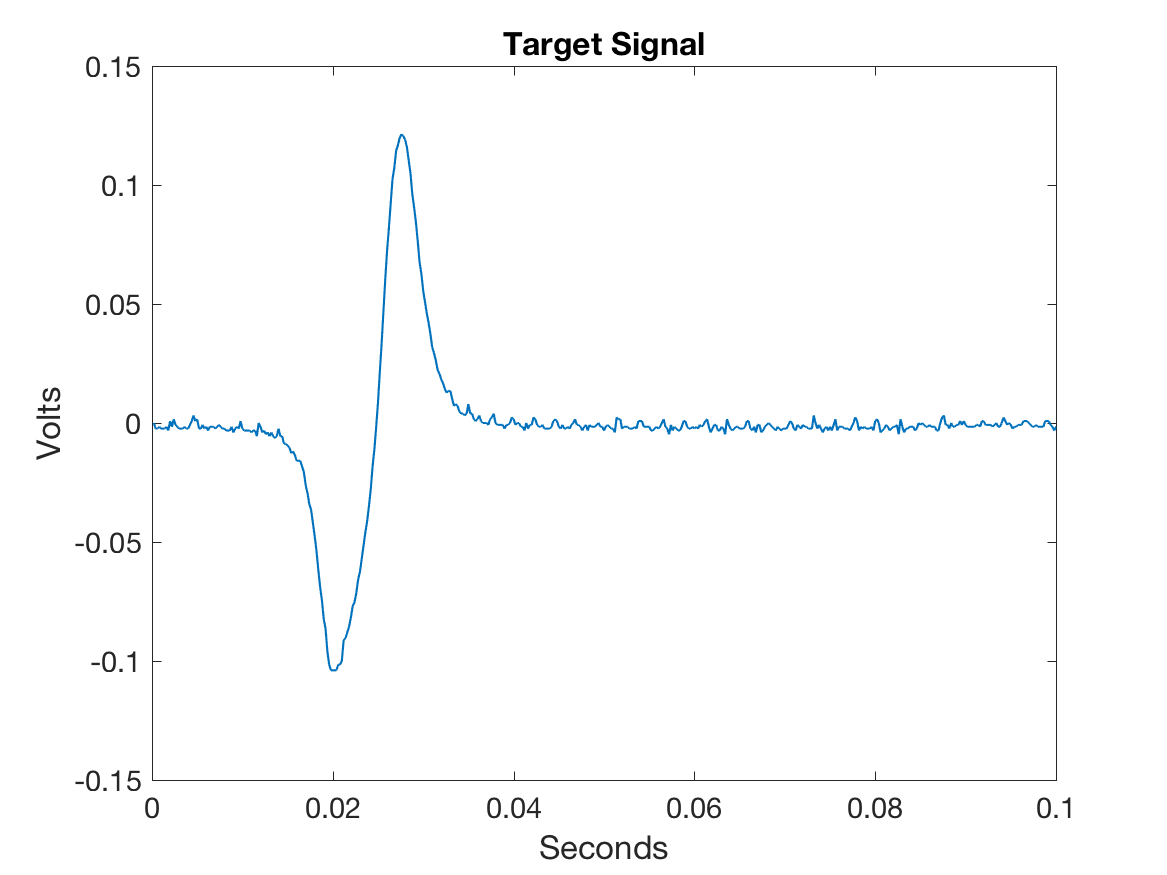
\includegraphics[width=8cm]{../matlab/plot5.png}
  \caption{Signal from prototype device}
  \label{fig:input}
  \end{figure}
Therefore we should
correlate our input signal with this signal to maximize the separation
from noise. To make sure this technique would suit our needs, a script
was created in MATLAB to illustrate the effects of the correlation.

First, the signal in Figure \,\ref{fig:input}. was modified by adding some noise, and appears in Figure \,\ref{fig:noisy}
\begin{figure}[h]
  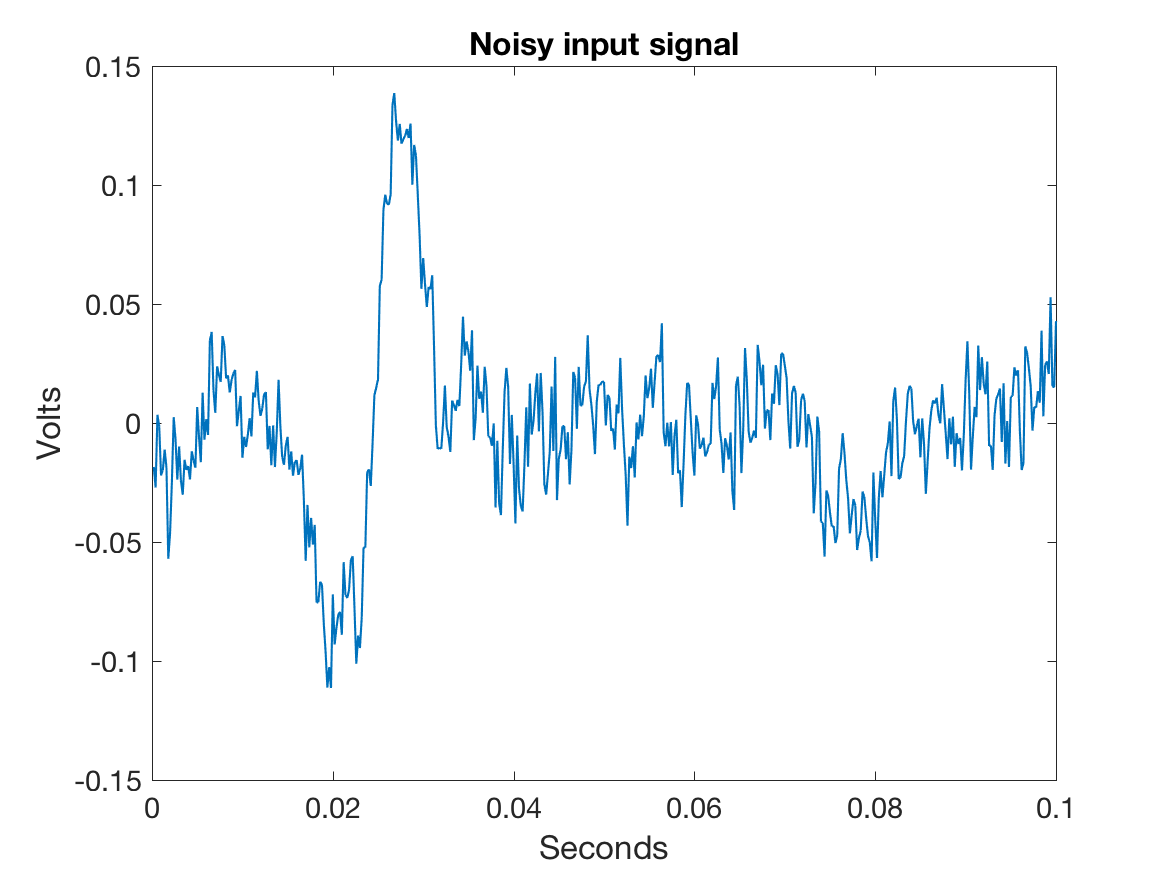
\includegraphics[width=8cm]{../matlab/plot1.png}
  \caption{Signal with simulated noise}
  \label{fig:noisy}
\end{figure}
Next, the signal was correlated with the signal in Figure \,\ref{fig:target}, and the resulting signal appears in Figure \,\ref{fig:correl}.

\begin{figure}[h]
  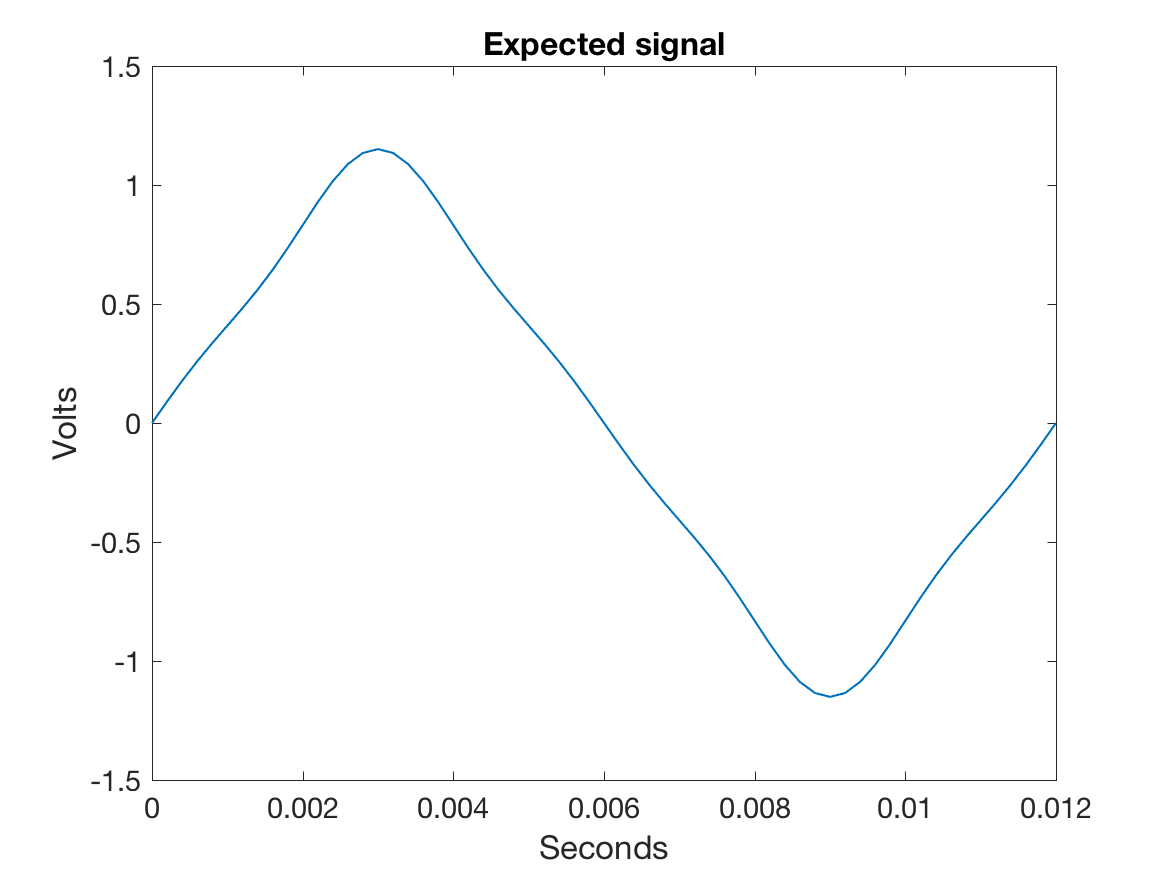
\includegraphics[width=8cm]{../matlab/plot2.png}
  \caption{Correlation target signal}
  \label{fig:target}
\end{figure}

\begin{figure}[h]
  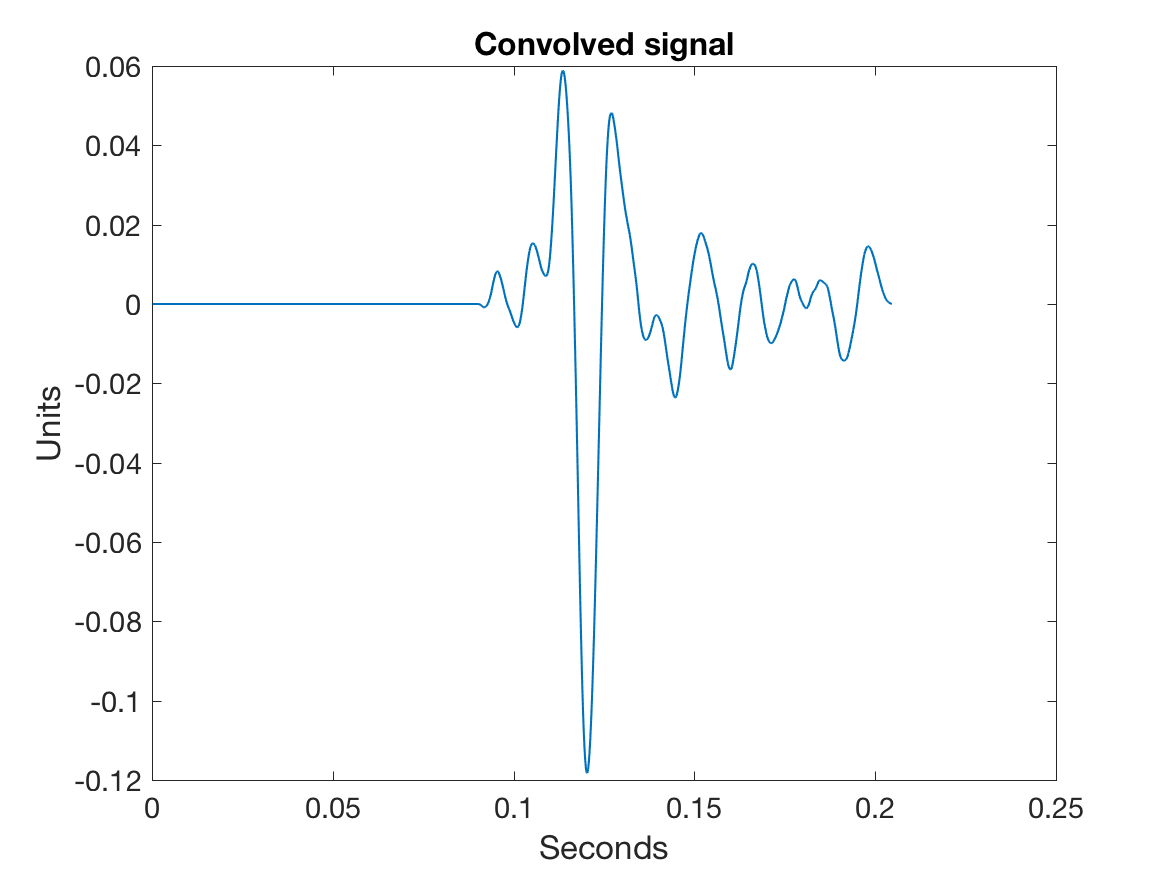
\includegraphics[width=8cm]{../matlab/plot3.png}
  \caption{Result of correlation}
  \label{fig:correl}
\end{figure}

Notice how Figure \,\ref{fig:correl} has several small bumps where the
target signal matched weakly with the noise, and also the very large
negative spike from where the target signal was lined up with the
pulse in the input signal. Unfortunately, the signal from the
uFluidics device can be either positive or negative, so further
processing is needed. To force both polarities to be positive, the
signal in Figure \,\ref{fig:correl} is squared, which also has the
effect of reducing the relative amplitude of the spikes from the noise
compared with the desired spike. Finally, the number of spikes above a
threshold value are counted, and the result appears in Figure
\,\ref{fig:result}.

\begin{figure}[h]
  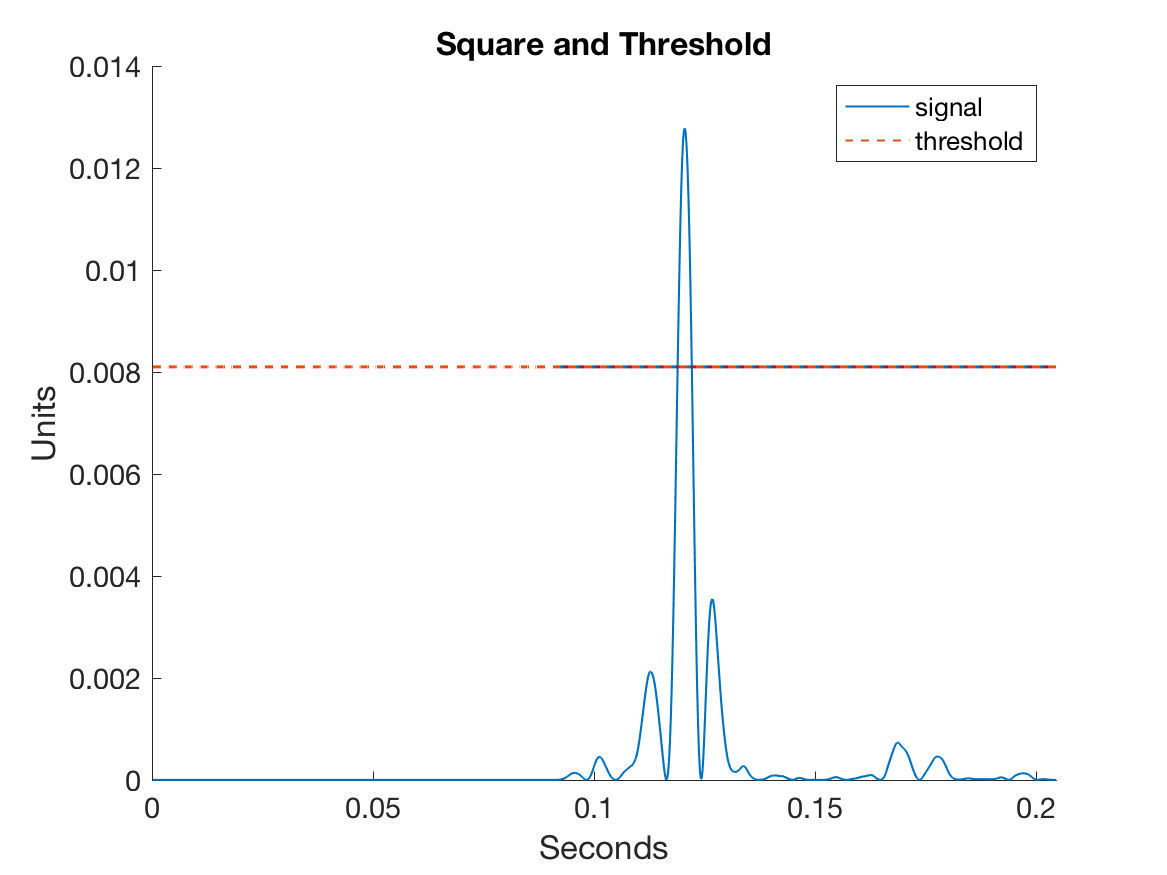
\includegraphics[width=8cm]{../matlab/plot4.png}
  \caption{Squared signal with threshold}
  \label{fig:result}
\end{figure}

\subsection{Software}

The DSP was programmed in C, with some functions, such as squaring and
thresholding, written in assembly. The processing is as above, with
some additional considerations for continuous processing. 256 samples
are read from the ADC and fed into a buffer, along with the previous
256 samples. Then, those 512 samples are correlated with the signal
from Fig. \,\ref{fig:target}, and the resulting signal is placed into
another buffer. Each sample in the buffer is squared, and then the 256
samples starting at sample number $256-61=195$ (256 - samples from the
previous sample period, 61 - number of samples in the target signal)
are fed to the threshold counting function, which counts the number of
times the signal crosses the threshold value going positive. The
threshold is only run on these samples so that a cell that generates a
signal between the two aquisition periods will still get counted.

\newpage
\bibliographystyle{ieeetr} \bibliography{dsp}{}

\end{document}
